\section{忙期服务过程 ($Q \to P$) 的详细推导}
\label{app:proof_lemma2}
%\addcontentsline{toc}{section}{忙期服务过程 ($Q \to P$) 的详细推导}


本附录旨在详细推导节点忙期服务过程的统计特性。具体而言，我们将建立一个吸收马尔可夫链模型，以刻画从忙期开始时刻的队列长度 $Q$ 演变为忙期结束时刻的队列长度 $P$ 的随机过程，并最终导出 $P$ 的概率生成函数（PGF）$G_P(z)$ 与 $Q$ 的 PGF $G_Q(z)$ 之间的解析关系。

\subsection{ 吸收马尔可夫链模型的构建}

为了描述忙期内节点队列长度的动态变化及忙期终止的随机性，我们定义二维状态随机过程 $\{ (L_t, K_t), t=0, 1, \dots \}$, 其中：
\begin{itemize}
	\item $L_t \in \{0, 1, \dots\}$ 表示节点在第 $t$ 次传输尝试\textbf{开始时}的剩余队列长度（不包含正在传输的那个数据包）。注意，若忙期开始时的总队列长度为 $Q$，则初始时刻 $L_0 = Q - 1$（因为 HoL 包已占用信道）。
	\item $K_t \in \{0, 1\}$ 表示信道状态指示变量。$K_t=1$ 表示节点处于忙期保持状态（即传输成功，继续发送）；$K_t=0$ 表示节点进入忙期终止状态（即发生碰撞或传输结束）。
\end{itemize}

如图 \ref{fig:absorbing_markov} 所示，该过程可建模为一个\textbf{吸收马尔可夫链（Absorbing Markov Chain）}，其状态空间划分为：
\begin{itemize}
	\item \textbf{瞬态（Transient States）} $\mathcal{S}_T = \{ (j, 1) \mid j \ge 0 \}$：表示节点正在成功传输数据包，且队列中仍有 $j$ 个数据包等待发送。只要系统处于瞬态，忙期就会持续。
	\item \textbf{吸收态（Absorbing States）} $\mathcal{S}_A = \{ (j, 0) \mid j \ge 0 \}$：表示由于信道碰撞或数据发送完毕，忙期终止。一旦进入该状态，过程停止，此时的 $L_t$ 即为忙期结束时的剩余队列长度 $P$。
\end{itemize}

\begin{figure}[htbp]
	\centering
	% 请确保图片路径和文件名正确
	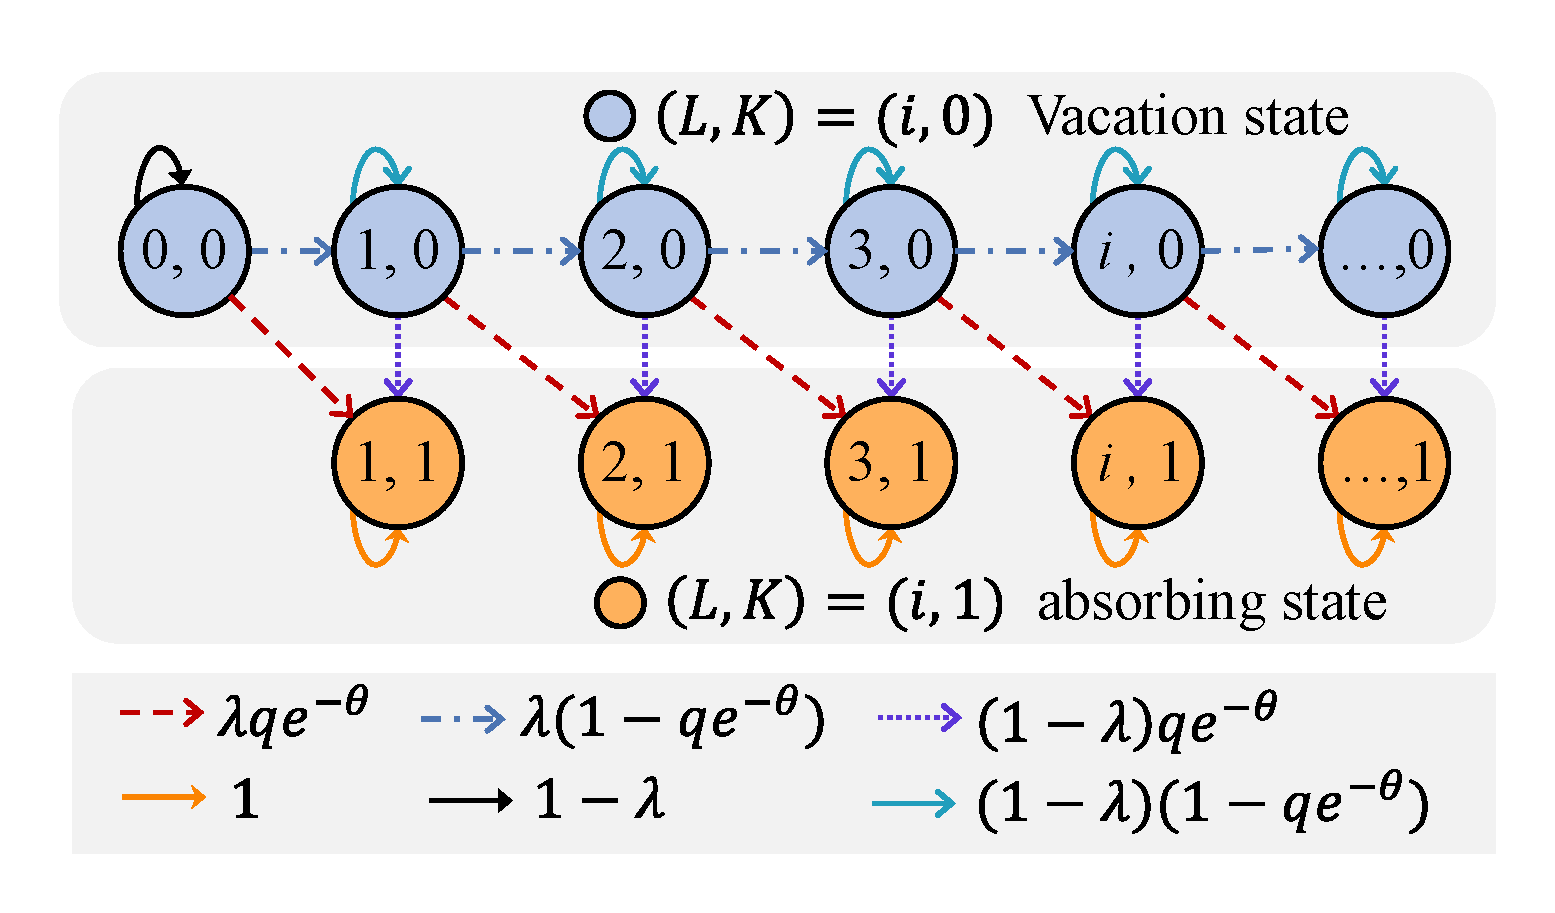
\includegraphics[width=0.8\textwidth]{figure/appdix/P2Q_Absorbing_Markov_chain.pdf}
	\caption{描述忙期内队列演化的吸收马尔可夫链状态转移图}
	\label{fig:absorbing_markov}
\end{figure}

\subsection{状态转移概率分析}

考虑系统当前处于瞬态 $(j, 1)$，即节点正在传输一个数据包，且缓存中还有 $j$ 个包。在一个时隙内，可能发生两类独立事件：
\begin{enumerate}
	\item \textbf{新数据包到达}：以概率 $\lambda$ 发生（服从伯努利过程）。
	\item \textbf{传输结果}：传输成功（其他 $n-1$ 个节点保持静默）的概率为 $e^{-\theta}$；传输失败（发生碰撞）的概率为 $1 - e^{-\theta}$。
\end{enumerate}

综合上述两个过程，下一时刻的状态转移存在以下四种情形：

\begin{enumerate}
	\item \textbf{成功传输且有新包到达}：概率为 $\lambda e^{-\theta}$。传输成功使得队列减 1，新包到达使得队列加 1，总长度不变。状态从 $(j, 1)$ 转移至 $(j, 1)$（自环）。
	\item \textbf{成功传输且无新包到达}：概率为 $(1-\lambda)e^{-\theta}$。传输成功使得队列减 1，无新包补充。状态从 $(j, 1)$ 转移至 $(j-1, 1)$。
	\item \textbf{传输失败且有新包到达}：概率为 $\lambda(1-e^{-\theta})$。发生碰撞导致忙期立即结束，但新包已进入缓存。状态从 $(j, 1)$ 被吸收至 $(j+1, 0)$。
	\item \textbf{传输失败且无新包到达}：概率为 $(1-\lambda)(1-e^{-\theta})$。发生碰撞导致忙期结束，且无新包。状态从 $(j, 1)$ 被吸收至 $(j, 0)$。
\end{enumerate}

\subsection{转移矩阵与基本解}

假设忙期开始时的初始队列长度为 $Q$。除去 $Q=1$ 的平凡情况（此时必然直接进入吸收态 $(0,0)$，即 $P=0$），对于 $Q \ge 2$ 的一般情况，系统从瞬态 $(Q-1, 1)$ 出发。
为了求解吸收概率，我们将状态空间截断至有限维度（例如最大队列长度为 $J$，令 $J \to \infty$），其标准形式的转移概率矩阵 $\mathbf{M}$ 可分块表示为：
\begin{equation}
	\mathbf{M} = 
	\left(
	\begin{array}{cc}
		\mathbf{T} & \mathbf{R} \\
		\mathbf{0} & \mathbf{I}
	\end{array}
	\right),
\end{equation}
其中：
\begin{itemize}
	\item $\mathbf{T}$ 是描述瞬态间转移的子矩阵（下双对角矩阵），元素 $t_{j,j} = \lambda e^{-\theta}$，$t_{j, j-1} = (1-\lambda)e^{-\theta}$。
	\item $\mathbf{R}$ 是描述从瞬态进入吸收态的子矩阵，元素 $r_{j, j+1} = \lambda(1-e^{-\theta})$，$r_{j, j} = (1-\lambda)(1-e^{-\theta})$。
\end{itemize}

根据吸收马尔可夫链理论，从任意瞬态 $s_i$ 出发最终被吸收态 $s_j$ 吸收的概率 $b_{ij}$ 由基本矩阵 $\mathbf{B} = (\mathbf{I} - \mathbf{T})^{-1} \mathbf{R}$ 给出。
通过求解该矩阵方程（利用 $\mathbf{T}$ 的下三角结构特性进行递归求解），我们可以得到从初始状态 $(Q-1, 1)$ 出发，最终停留在各个吸收态 $(k, 0)$ 的概率，即条件概率 $\Pr\{P=k \mid Q\}$。

经过代数运算，我们得到如下解析解：

\begin{enumerate}
	\item 当 $Q=1$ 时：
	\begin{equation}
		\Pr\{P=0 \mid Q=1\} = 1.
	\end{equation}
	
	\item 当 $Q \ge 2$ 时，对于 $0 \le k \le Q$：
	\begin{equation}
		\Pr\{P=k \mid Q\} = 
		\begin{cases}
			\left[ \frac{(1-\lambda)e^{-\theta}}{1-\lambda e^{-\theta}} \right]^{Q-1}, & k=0 \\
			\frac{(1-\lambda)(1-e^{-\theta})}{1-\lambda e^{-\theta}} \left[ \frac{(1-\lambda)e^{-\theta}}{1-\lambda e^{-\theta}} \right]^{Q-2}, & k=1 \\
			\dots & \vdots \\
			\frac{\lambda(1-e^{-\theta})}{1-\lambda e^{-\theta}}, & k=Q
		\end{cases}
	\end{equation}
\end{enumerate}

\subsection{PGF 关系的建立}

尽管上述条件概率分布形式较为复杂，但在大系统极限下（即 $n \to \infty$ 导致 $\lambda \to 0$），我们可以利用 PGF 的性质获得更简洁的关系。
回顾 $P$ 的物理意义：它是 $Q$ 经过一系列成功传输（队列减1）和新包到达（队列加1）操作后，被碰撞（停止）截断时的状态。
利用 PGF 的变换性质，可以证明 $G_P(z)$ 与 $G_Q(z)$ 满足如下线性关系：
\begin{equation}
	\label{eq:pgf_P_appendix}
	G_P(z) = G_Q(e^{-\theta}) + \frac{1 - e^{-\theta}}{e^{-\theta} - z} \left[ G_Q(e^{-\theta}) - G_Q(z) \right].
\end{equation}
该式直观地反映了忙期过程对队列分布的过滤作用：$e^{-\theta}$ 项对应于传输成功的概率流，而分母中的 $e^{-\theta}-z$ 项则体现了队列长度随时间步的演化特征。这一结论直接支持了正文中关于 $p_0 = G_P(0)$ 的闭式求解。
